\documentclass[10pt,a4paper,titlepage]{article}
\usepackage{amsmath}
\usepackage{amsfonts}
\usepackage{amssymb}
\usepackage[OT1]{fontenc}
\usepackage[utf8]{inputenc}
\usepackage[russian]{babel}
\usepackage{listings}
\usepackage{graphicx}
\usepackage{hyperref}
\hypersetup{
    colorlinks,
    citecolor=black,
    filecolor=black,
    linkcolor=black,
    urlcolor=blue
}
\begin{document}

%--titlepage-----
\begin{titlepage}
  \begin{center}
    \large
    \textbf{Федеральное государственное автономное образовательное учреждение\\
    Высшего профессионального образования}

    \vspace{0.25cm}

    Санкт-Петербургский политехнический университет
    \vspace{0.25cm}
    
    Институт компьютерных наук и технологий
    \vspace{0.25cm}
    
    Кафедра компьютерных систем и программных технологий
    \vfill

    \textbf{\textsc{Лабораторная работа №3}}\\[5mm]
    
    {\LARGE Утилита для исследования сети и сканер портов Nmap}
  \bigskip
    
\end{center}
\vfill

\newlength{\ML}
\settowidth{\ML}{«\underline{\hspace{0.7cm}}» \underline{\hspace{2cm}}}
\hfill\begin{minipage}{0.4\textwidth}
  Выполнил студент\\ группы 53501/3\\
  \underline{\hspace{\ML}} П.\,П.~Жук\\
  «\underline{\hspace{0.7cm}}» \underline{\hspace{2cm}} 2016 г.
\end{minipage}%
\bigskip

\hfill\begin{minipage}{0.4\textwidth}
  Проверил преподаватель\\
  \underline{\hspace{\ML}}\\ К.\,Д.~Вылегжанина\\
  «\underline{\hspace{0.7cm}}» \underline{\hspace{2cm}} 2016 г.
\end{minipage}%
\vfill

\begin{center}
  Санкт-Петербург\\ 2016 г.
\end{center}
\end{titlepage}
%---------------

\tableofcontents
\newpage

\section{Цель работы}
Изучить основные аспекты работы с утилитой Nmap на различных примерах.

\section{Задание}
\begin{enumerate}
	\item Провести поиск активных хостов.
    \item Определить открытые порты.
    \item Определить версии сервисов.
    \item Изучить файлы nmap-services, nmap-os-db, nmap-service-probes
    \item Добавить новую сигнатуру службы в файл nmap-service-probes.
    \item Сохранить вывод утилиты в формате xml.
    \item Исследвать различные этапы и режимы работы Nmap с использованием утилиты Wireshark.
    \item Просканировать виртуальную машину Metasploitable2 используя утилиту db\_nmap из состава metasploit-framework.
    \item Выбрать пять записей из файла nmap-service-probes и описать их работу.
    \item Выбрать один скрипт из состава Nmap и описать его работу.
\end{enumerate}

\section{Ход работы}
Для проведения лабораторной работы было создано две виртуальные машины, объединенные в общую  сеть. Metasploitable2 - виртуальная машина, намеренно содержащая ряд уязвимостей. Kali Linux - виртуальная машина, необходима для сканирования и поиска уязвимостей на первой виртуальной машине. Определим IP-адреса виртуальных машин:

\begin{verbatim}
root@kali:~# ifconfig
eth0: flags=4163<UP,BROADCAST,RUNNING,MULTICAST>  mtu 1500
        inet 192.168.226.135  netmask 255.255.255.0  broadcast 192.168.226.255
        inet6 fe80::20c:29ff:fe48:9c2a  prefixlen 64  scopeid 0x20<link>
        ether 00:0c:29:48:9c:2a  txqueuelen 1000  (Ethernet)
        RX packets 81  bytes 11060 (10.8 KiB)
        RX errors 0  dropped 0  overruns 0  frame 0
        TX packets 74  bytes 6535 (6.3 KiB)
        TX errors 0  dropped 0 overruns 0  carrier 0  collisions 0

\end{verbatim}

\begin{figure}[h]	\center{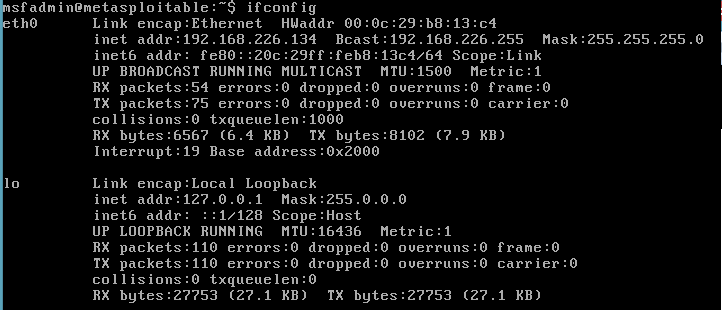
\includegraphics[width=1.2\linewidth]{pics/1.png}}
\caption{IP-адрес Metasploitable2}
\label{ris:image1}
\end{figure}

Виртуальная машина с ОС Metasploitable2 имеет адрес 192.168.226.134, вторая (с Kali Linux) имеет адрес 192.168.226.135.

Для проверки работоспособности сети "пропингуем" виртуальные машины:

\begin{verbatim}
root@kali:~# ping 192.168.226.134
PING 192.168.226.134 (192.168.226.134) 56(84) bytes of data.
64 bytes from 192.168.226.134: icmp_seq=1 ttl=64 time=0.230 ms
64 bytes from 192.168.226.134: icmp_seq=2 ttl=64 time=0.384 ms
64 bytes from 192.168.226.134: icmp_seq=3 ttl=64 time=0.376 ms
64 bytes from 192.168.226.134: icmp_seq=4 ttl=64 time=0.410 ms
^C
--- 192.168.226.134 ping statistics ---
4 packets transmitted, 4 received, 0% packet loss, time 2999ms
rtt min/avg/max/mdev = 0.230/0.350/0.410/0.070 ms
\end{verbatim}

\begin{figure}[h]	\center{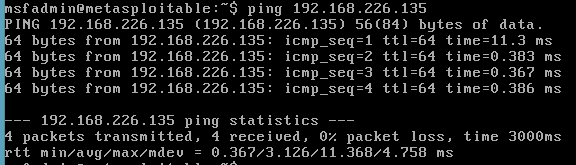
\includegraphics[width=1.1\linewidth]{pics/2.png}}
\caption{Пингуем Kali Linux}
\label{ris:image2}
\end{figure}

Пакеты проходят, значит сеть работоспособна.

\subsection{Провести поиск активных хостов}
Для поиска активных хостов используется флаг -sP. При этом также нужно указать адрес подсети, который в данном случае будет 192.168.226.* .

\begin{verbatim}
root@kali:~# nmap -sP 192.168.226.*

Starting Nmap 7.01 ( https://nmap.org ) at 2016-06-14 09:54 EDT
Nmap scan report for 192.168.226.1
Host is up (0.00018s latency).
MAC Address: 00:50:56:C0:00:08 (VMware)
Nmap scan report for 192.168.226.2
Host is up (0.000098s latency).
MAC Address: 00:50:56:E5:ED:96 (VMware)
Nmap scan report for 192.168.226.134
Host is up (0.00035s latency).
MAC Address: 00:0C:29:B8:13:C4 (VMware)
Nmap scan report for 192.168.226.254
Host is up (0.00020s latency).
MAC Address: 00:50:56:F2:AB:24 (VMware)
Nmap scan report for 192.168.226.135
Host is up.
Nmap done: 256 IP addresses (5 hosts up) scanned in 2.01 seconds
\end{verbatim}

В результате было найдено 5 активных хостов, среди которых присутсвует и Metasploitable2.

\subsection{Определить открытые порты}
Для определения открытых портов утилите необходимо передать адрес хоста. Простой командой nmap <цель сканирования> будет произведено сканирование более чем 1660 TCP портов на <целевой машине>. 
\begin{verbatim}
root@kali:~# nmap 192.168.226.134

Starting Nmap 7.01 ( https://nmap.org ) at 2016-06-14 10:27 EDT
Nmap scan report for 192.168.226.134
Host is up (0.00013s latency).
Not shown: 978 closed ports
PORT     STATE SERVICE
21/tcp   open  ftp
22/tcp   open  ssh
23/tcp   open  telnet
25/tcp   open  smtp
53/tcp   open  domain
80/tcp   open  http
111/tcp  open  rpcbind
139/tcp  open  netbios-ssn
445/tcp  open  microsoft-ds
512/tcp  open  exec
513/tcp  open  login
514/tcp  open  shell
1099/tcp open  rmiregistry
1524/tcp open  ingreslock
2049/tcp open  nfs
2121/tcp open  ccproxy-ftp
3306/tcp open  mysql
5432/tcp open  postgresql
5900/tcp open  vnc
6000/tcp open  X11
6667/tcp open  irc
8180/tcp open  unknown
MAC Address: 00:0C:29:B8:13:C4 (VMware)

Nmap done: 1 IP address (1 host up) scanned in 0.37 seconds

\end{verbatim}
В результате мы получили адреса открытых портов и названия соответсвующих им сервисов.

\subsection{Определить версии сервисов}
Для определения вресии сервиса используется флаг -sV.
\begin{verbatim}
root@kali:~# nmap -sV 192.168.226.134

Starting Nmap 7.01 ( https://nmap.org ) at 2016-06-14 10:40 EDT
Nmap scan report for 192.168.226.134
Host is up (0.00015s latency).
Not shown: 978 closed ports
PORT     STATE SERVICE     VERSION
21/tcp   open  ftp         vsftpd 2.3.4
22/tcp   open  ssh         OpenSSH 4.7p1 Debian 8ubuntu1 (protocol 2.0)
23/tcp   open  telnet      Linux telnetd
25/tcp   open  smtp        Postfix smtpd
53/tcp   open  domain      ISC BIND 9.4.2
80/tcp   open  http        Apache httpd 2.2.8 ((Ubuntu) DAV/2)
111/tcp  open  rpcbind     2 (RPC #100000)
139/tcp  open  netbios-ssn Samba smbd 3.X (workgroup: WORKGROUP)
445/tcp  open  netbios-ssn Samba smbd 3.X (workgroup: WORKGROUP)
512/tcp  open  exec        netkit-rsh rexecd
513/tcp  open  login?
514/tcp  open  tcpwrapped
1099/tcp open  rmiregistry GNU Classpath grmiregistry
1524/tcp open  shell       Metasploitable root shell
2049/tcp open  nfs         2-4 (RPC #100003)
2121/tcp open  ftp         ProFTPD 1.3.1
3306/tcp open  mysql       MySQL 5.0.51a-3ubuntu5
5432/tcp open  postgresql  PostgreSQL DB 8.3.0 - 8.3.7
5900/tcp open  vnc         VNC (protocol 3.3)
6000/tcp open  X11         (access denied)
6667/tcp open  irc         Unreal ircd
8180/tcp open  unknown
MAC Address: 00:0C:29:B8:13:C4 (VMware)
Service Info: Hosts:  metasploitable.localdomain, localhost, irc.Metasploitable.LAN; OSs: Unix, Linux; CPE: cpe:/o:linux:linux_kernel

Service detection performed. Please report any incorrect results at https://nmap.org/submit/ .
Nmap done: 1 IP address (1 host up) scanned in 147.51 seconds
\end{verbatim}

\pagebreak
\subsection{Изучить файлы nmap-services, nmap-os-db, nmap-service-probes}
Служебные файлы для nmap можно найти в директории "/usr/share/nmap".

Файл  \textbf{nmap-services} описывает назначение стандартных портов. Каждая запись имеет следующий вид: имя\_сервиса, номер\_порта/протокол, вероятность\_открытости\_порта, опциональный\_комментарий.
			
Для известных, зарезервированных номеров портов, файл содержит подробное описание. Для незакрепленных портов также есть записи, но с "unknown" в качестве имени:

\begin{verbatim}
fln-spx	221/udp	0.000577	# Berkeley rlogind with SPX auth
rsh-spx	222/tcp	0.000941	# Berkeley rshd with SPX auth
rsh-spx	222/udp	0.000774	# Berkeley rshd with SPX auth
cdc	223/tcp	0.000125	# Certificate Distribution Center
cdc	223/udp	0.000346	# Certificate Distribution Center
masqdialer	224/tcp	0.000025
unknown	225/tcp	0.000100
unknown	225/udp	0.000330
unknown	226/tcp	0.000013
unknown	228/tcp	0.000013
\end{verbatim}
			
Файл  \textbf{nmap-os-db} содержит примеры ответов различных операционных систем при сканировании. Это необходимо для того, что бы узнать какая операционная система находится на данном хосте. Пример:

			\begin{verbatim}
				MatchPoints
				SEQ(SP=25%GCD=75%ISR=25%TI=100%CI=50%II=100%SS=80%TS=100)
				OPS(O1=20%O2=20%O3=20%O4=20%O5=20%O6=20)
				WIN(W1=15%W2=15%W3=15%W4=15%W5=15%W6=15)
				ECN(R=100%DF=20%T=15%TG=15%W=15%O=15%CC=100%Q=20)
			\end{verbatim}
			
			Для вывода информации об ОС на хосте используется ключ -O:
			
			\begin{verbatim}
root@kali:~# nmap -O 192.168.226.134

Starting Nmap 7.01 ( https://nmap.org ) at 2016-06-14 11:04 EDT
Nmap scan report for 192.168.226.134
Host is up (0.00036s latency).
Not shown: 978 closed ports
PORT     STATE SERVICE
21/tcp   open  ftp
22/tcp   open  ssh
23/tcp   open  telnet
25/tcp   open  smtp
53/tcp   open  domain
80/tcp   open  http
111/tcp  open  rpcbind
139/tcp  open  netbios-ssn
445/tcp  open  microsoft-ds
512/tcp  open  exec
513/tcp  open  login
514/tcp  open  shell
1099/tcp open  rmiregistry
1524/tcp open  ingreslock
2049/tcp open  nfs
2121/tcp open  ccproxy-ftp
3306/tcp open  mysql
5432/tcp open  postgresql
5900/tcp open  vnc
6000/tcp open  X11
6667/tcp open  irc
8180/tcp open  unknown
MAC Address: 00:0C:29:B8:13:C4 (VMware)
Device type: general purpose
Running: Linux 2.6.X
OS CPE: cpe:/o:linux:linux_kernel:2.6
OS details: Linux 2.6.9 - 2.6.33
Network Distance: 1 hop

OS detection performed. Please report any incorrect results at https://nmap.org/submit/ .
Nmap done: 1 IP address (1 host up) scanned in 1.76 seconds

			\end{verbatim}
Видно, что на Metasploitable2 используется Linux с версией ядра 2.6.

Файл \textbf{nmap-service-probes} содержит сигнатуры для определения сервисов, прослушивающих тот или иной порт. Понимание устройства этого файла позволит добавить сигнатуру для, например, собственного сервиса. Каждая запись в данном файле определяется одной сторокой. Строки, начинающиеся с хэша (\#) рассматриваются как комментарии и игнорируются. Пустые строки игнорируются также. Другие строки должны содержать одну из директив, описанных ниже.

\begin{itemize}
\item Probe <protocol> <probename> <probestring> \\ Директива Probe содержит строку, необходимую для отправки при распознавании сервиса.
\item match <service> <pattern> [<versioninfo>]\\
Директива match необходима при распознавании сервиса на основе ответов на строку, отправленную предыдущей директивой Probe.
\item ports <portlist>\\
Директива ports содержит порты сервиса.
\item rarity <value between 1 and 9> \\
Директива rarity указывает частоту, с которой от сервиса можно ожидать возвращения корректных результатов.
\item некоторые другие
\end{itemize}
Пример из файла nmap-service-probes
\begin{verbatim}
# Microsoft ActiveSync Version 3.7 Build 3083 (It's used for syncing
# my ipaq it disappears when you remove the ipaq.)
match activesync m|^.\0\x01\0[^\0]\0[^\0]\0[^\0]\0[^\0]\0[^\0]\0.*\0\0\0$|s p/Microsoft ActiveSync/ o/Windows/ cpe:/a:microsoft:activesync/ cpe:/o:microsoft:windows/a
match activesync m|^\(\0\0\0\x02\0\0\0\x03\0\0\0\+\0\0\x003\0\0\0\0\0\0\0\x04\0\0`\x01\0\0\xff\0\0\0\0\0\0\0\0\0\0\0$|s p/Citrix ActiveSync/ o/Windows/ cpe:/o:microsoft:windows/a
\end{verbatim}	

\subsection{Добавить новую сигнатуру службы в файл nmap-service-probes}
Создадим простой сервер, который мы будем идентифицировать с помощью утилиты nmap.
\begin{verbatim}
#include <sys/socket.h>
#include <stdio.h>
#include <unistd.h>
#include <stdlib.h>
#include <string.h>
#include <netinet/in.h>
#include <arpa/inet.h>

#define PORT 8133

int main(int argc, char** argv)
{
char str[100];
char *msg="Hello";
struct sockaddr_in server_addr;

server_addr.sin_family = AF_INET;
server_addr.sin_port = htons(PORT);
server_addr.sin_addr.s_addr = htonl(INADDR_ANY);

int listener = socket(AF_INET,SOCK_STREAM,0);

if(listener < 0) {
    perror("Can't create socket.");
    exit(1);
}

if(bind(listener,(struct sockaddr *) &server_addr,sizeof(server_addr)) < 0) {
    perror("Can't bind socket.");
    exit(1);
}

if(listen(listener,5)) {
    perror("Erro while listening:");
    exit(1);
}

int client = accept(listener,NULL,NULL);

while(1)
{
    bzero( str, 100);
    recv(client,str, 100, 0);
    printf("Message from client - %s",str);
    send(client, msg, (int)strlen(msg), 0);
}

return 0;
}
\end{verbatim}

Сервер слушает порт 8133 и на входящее сообщение отправляет "Hello".\\
		
Для определения данного сервиса, добавим в файл nmap-service-probes следующие строки:
\begin{verbatim}
	Probe TCP testServer q|Hi|
	rarity 1
	ports 8133
	match testServer m|Hello|
\end{verbatim}
		
В данных строках мы описываем, что серсиву с именем testServer мы посылаем сообщение Hi на порт 8133 и ожидаем в ответ сообщение Hello.\\
		
Запустим на испытуемой виртуальной машине данный сервер и попробуем определить его при помощи утилиты nmap:
		\begin{verbatim}
root@kali:~# nmap 192.168.226.134

Starting Nmap 7.01 ( https://nmap.org ) at 2016-06-14 12:06 EDT
Nmap scan report for 192.168.226.134
Host is up (0.00014s latency).
Not shown: 977 closed ports
PORT     STATE SERVICE
21/tcp   open  ftp
22/tcp   open  ssh
23/tcp   open  telnet
25/tcp   open  smtp
53/tcp   open  domain
80/tcp   open  http
111/tcp  open  rpcbind
139/tcp  open  netbios-ssn
445/tcp  open  microsoft-ds
512/tcp  open  exec
513/tcp  open  login
514/tcp  open  shell
1099/tcp open  rmiregistry
1524/tcp open  ingreslock
2049/tcp open  nfs
2121/tcp open  ccproxy-ftp
3306/tcp open  mysql
5432/tcp open  postgresql
5900/tcp open  vnc
6000/tcp open  X11
6667/tcp open  irc
8133/tcp open  testServer
8180/tcp open  unknown
MAC Address: 00:0C:29:B8:13:C4 (VMware)

Nmap done: 1 IP address (1 host up) scanned in 0.21 seconds
\end{verbatim}

Видно, что утилита корректно определила наш сервер.

\subsection{Сохранить вывод утилиты в формате xml}
Для сохранения вывода nmap в файле в формате xml необходимо указать флаг -oX и имя файла.
\begin{verbatim}
root@kali:~# nmap 192.168.226.134 -oX xml_output.xml
\end{verbatim}
Содержимое файла \textbf{xml\_output.xml} приведено ниже.
\begin{verbatim}
<?xml version="1.0" encoding="UTF-8"?>
<!DOCTYPE nmaprun>
<?xml-stylesheet href="file:///usr/bin/../share/nmap/nmap.xsl" type="text/xsl"?>
<!-- Nmap 7.01 scan initiated Tue Jun 14 12:27:40 2016 as: nmap -oX xml_output.xml 192.168.226.134 -->
<nmaprun scanner="nmap" args="nmap -oX xml_output.xml 192.168.226.134" start="1465921660" startstr="Tue Jun 14 12:27:40 2016" version="7.01" xmloutputversion="1.04">
<scaninfo type="syn" protocol="tcp" numservices="1000" services="1,3-4,6-7,9,13,17,19-26,30,32-33,37,42-43,49,53,70,79-85,88-90,99-100,106,109-111,113,119,125,135,139,143-144,146,161,163,179,199,211-212,222,254-256,259,264,280,301,306,311,340,366,389,406-407,416-417,425,427,443-445,458,464-465,481,497,500,512-515,524,541,543-545,548,554-555,563,587,593,616-617,625,631,636,646,648,666-668,683,687,691,700,705,711,714,720,722,726,749,765,777,783,787,800-801,808,843,873,880,888,898,900-903,911-912,981,987,990,992-993,995,999-1002,1007,1009-1011,1021-1100,1102,1104-1108,1110-1114,1117,1119,1121-1124,1126,1130-1132,1137-1138,1141,1145,1147-1149,1151-1152,1154,1163-1166,1169,1174-1175,1183,1185-1187,1192,1198-1199,1201,1213,1216-1218,1233-1234,1236,1244,1247-1248,1259,1271-1272,1277,1287,1296,1300-1301,1309-1311,1322,1328,1334,1352,1417,1433-1434,1443,1455,1461,1494,1500-1501,1503,1521,1524,1533,1556,1580,1583,1594,1600,1641,1658,1666,1687-1688,1700,1717-1721,1723,1755,1761,1782-1783,1801,1805,1812,1839-1840,1862-1864,1875,1900,1914,1935,1947,1971-1972,1974,1984,1998-2010,2013,2020-2022,2030,2033-2035,2038,2040-2043,2045-2049,2065,2068,2099-2100,2103,2105-2107,2111,2119,2121,2126,2135,2144,2160-2161,2170,2179,2190-2191,2196,2200,2222,2251,2260,2288,2301,2323,2366,2381-2383,2393-2394,2399,2401,2492,2500,2522,2525,2557,2601-2602,2604-2605,2607-2608,2638,2701-2702,2710,2717-2718,2725,2800,2809,2811,2869,2875,2909-2910,2920,2967-2968,2998,3000-3001,3003,3005-3007,3011,3013,3017,3030-3031,3052,3071,3077,3128,3168,3211,3221,3260-3261,3268-3269,3283,3300-3301,3306,3322-3325,3333,3351,3367,3369-3372,3389-3390,3404,3476,3493,3517,3527,3546,3551,3580,3659,3689-3690,3703,3737,3766,3784,3800-3801,3809,3814,3826-3828,3851,3869,3871,3878,3880,3889,3905,3914,3918,3920,3945,3971,3986,3995,3998,4000-4006,4045,4111,4125-4126,4129,4224,4242,4279,4321,4343,4443-4446,4449,4550,4567,4662,4848,4899-4900,4998,5000-5004,5009,5030,5033,5050-5051,5054,5060-5061,5080,5087,5100-5102,5120,5190,5200,5214,5221-5222,5225-5226,5269,5280,5298,5357,5405,5414,5431-5432,5440,5500,5510,5544,5550,5555,5560,5566,5631,5633,5666,5678-5679,5718,5730,5800-5802,5810-5811,5815,5822,5825,5850,5859,5862,5877,5900-5904,5906-5907,5910-5911,5915,5922,5925,5950,5952,5959-5963,5987-5989,5998-6007,6009,6025,6059,6100-6101,6106,6112,6123,6129,6156,6346,6389,6502,6510,6543,6547,6565-6567,6580,6646,6666-6669,6689,6692,6699,6779,6788-6789,6792,6839,6881,6901,6969,7000-7002,7004,7007,7019,7025,7070,7100,7103,7106,7200-7201,7402,7435,7443,7496,7512,7625,7627,7676,7741,7777-7778,7800,7911,7920-7921,7937-7938,7999-8002,8007-8011,8021-8022,8031,8042,8045,8080-8090,8093,8099-8100,8180-8181,8192-8194,8200,8222,8254,8290-8292,8300,8333,8383,8400,8402,8443,8500,8600,8649,8651-8652,8654,8701,8800,8873,8888,8899,8994,9000-9003,9009-9011,9040,9050,9071,9080-9081,9090-9091,9099-9103,9110-9111,9200,9207,9220,9290,9415,9418,9485,9500,9502-9503,9535,9575,9593-9595,9618,9666,9876-9878,9898,9900,9917,9929,9943-9944,9968,9998-10004,10009-10010,10012,10024-10025,10082,10180,10215,10243,10566,10616-10617,10621,10626,10628-10629,10778,11110-11111,11967,12000,12174,12265,12345,13456,13722,13782-13783,14000,14238,14441-14442,15000,15002-15004,15660,15742,16000-16001,16012,16016,16018,16080,16113,16992-16993,17877,17988,18040,18101,18988,19101,19283,19315,19350,19780,19801,19842,20000,20005,20031,20221-20222,20828,21571,22939,23502,24444,24800,25734-25735,26214,27000,27352-27353,27355-27356,27715,28201,30000,30718,30951,31038,31337,32768-32785,33354,33899,34571-34573,35500,38292,40193,40911,41511,42510,44176,44442-44443,44501,45100,48080,49152-49161,49163,49165,49167,49175-49176,49400,49999-50003,50006,50300,50389,50500,50636,50800,51103,51493,52673,52822,52848,52869,54045,54328,55055-55056,55555,55600,56737-56738,57294,57797,58080,60020,60443,61532,61900,62078,63331,64623,64680,65000,65129,65389"/>
<verbose level="0"/>
<debugging level="0"/>
<host starttime="1465921660" endtime="1465921660"><status state="up" reason="arp-response" reason_ttl="0"/>
<address addr="192.168.226.134" addrtype="ipv4"/>
<address addr="00:0C:29:B8:13:C4" addrtype="mac" vendor="VMware"/>
<hostnames>
</hostnames>
<ports><extraports state="closed" count="978">
<extrareasons reason="resets" count="978"/>
</extraports>
<port protocol="tcp" portid="21"><state state="open" reason="syn-ack" reason_ttl="64"/><service name="ftp" method="table" conf="3"/></port>
<port protocol="tcp" portid="22"><state state="open" reason="syn-ack" reason_ttl="64"/><service name="ssh" method="table" conf="3"/></port>
<port protocol="tcp" portid="23"><state state="open" reason="syn-ack" reason_ttl="64"/><service name="telnet" method="table" conf="3"/></port>
<port protocol="tcp" portid="25"><state state="open" reason="syn-ack" reason_ttl="64"/><service name="smtp" method="table" conf="3"/></port>
<port protocol="tcp" portid="53"><state state="open" reason="syn-ack" reason_ttl="64"/><service name="domain" method="table" conf="3"/></port>
<port protocol="tcp" portid="80"><state state="open" reason="syn-ack" reason_ttl="64"/><service name="http" method="table" conf="3"/></port>
<port protocol="tcp" portid="111"><state state="open" reason="syn-ack" reason_ttl="64"/><service name="rpcbind" method="table" conf="3"/></port>
<port protocol="tcp" portid="139"><state state="open" reason="syn-ack" reason_ttl="64"/><service name="netbios-ssn" method="table" conf="3"/></port>
<port protocol="tcp" portid="445"><state state="open" reason="syn-ack" reason_ttl="64"/><service name="microsoft-ds" method="table" conf="3"/></port>
<port protocol="tcp" portid="512"><state state="open" reason="syn-ack" reason_ttl="64"/><service name="exec" method="table" conf="3"/></port>
<port protocol="tcp" portid="513"><state state="open" reason="syn-ack" reason_ttl="64"/><service name="login" method="table" conf="3"/></port>
<port protocol="tcp" portid="514"><state state="open" reason="syn-ack" reason_ttl="64"/><service name="shell" method="table" conf="3"/></port>
<port protocol="tcp" portid="1099"><state state="open" reason="syn-ack" reason_ttl="64"/><service name="rmiregistry" method="table" conf="3"/></port>
<port protocol="tcp" portid="1524"><state state="open" reason="syn-ack" reason_ttl="64"/><service name="ingreslock" method="table" conf="3"/></port>
<port protocol="tcp" portid="2049"><state state="open" reason="syn-ack" reason_ttl="64"/><service name="nfs" method="table" conf="3"/></port>
<port protocol="tcp" portid="2121"><state state="open" reason="syn-ack" reason_ttl="64"/><service name="ccproxy-ftp" method="table" conf="3"/></port>
<port protocol="tcp" portid="3306"><state state="open" reason="syn-ack" reason_ttl="64"/><service name="mysql" method="table" conf="3"/></port>
<port protocol="tcp" portid="5432"><state state="open" reason="syn-ack" reason_ttl="64"/><service name="postgresql" method="table" conf="3"/></port>
<port protocol="tcp" portid="5900"><state state="open" reason="syn-ack" reason_ttl="64"/><service name="vnc" method="table" conf="3"/></port>
<port protocol="tcp" portid="6000"><state state="open" reason="syn-ack" reason_ttl="64"/><service name="X11" method="table" conf="3"/></port>
<port protocol="tcp" portid="6667"><state state="open" reason="syn-ack" reason_ttl="64"/><service name="irc" method="table" conf="3"/></port>
<port protocol="tcp" portid="8180"><state state="open" reason="syn-ack" reason_ttl="64"/><service name="unknown" method="table" conf="3"/></port>
</ports>
<times srtt="140" rttvar="21" to="100000"/>
</host>
<runstats><finished time="1465921660" timestr="Tue Jun 14 12:27:40 2016" elapsed="0.24" summary="Nmap done at Tue Jun 14 12:27:40 2016; 1 IP address (1 host up) scanned in 0.24 seconds" exit="success"/><hosts up="1" down="0" total="1"/>
</runstats>
</nmaprun>
\end{verbatim}

Также поддерживаются некоторые другие форматы, для которых определены соответсвующие флаги: -oS, -oG, -oN , -oA.

\subsection{Исследвать различные этапы и режимы работы Nmap с использованием утилиты Wireshark}
Wireshark - программа-анализатор трафика для компьютерных сетей Ethernet. Если, после запуска Wireshark, запусть сканирование nmap, то мы сможем проанализировать пакеты, посылаемые nmap.\\

При сканировании сети на наличие активных хостов утилита nmap обращается к DNS серверу для получения доступных узлов в данной подсети:

\begin{verbatim}
626	5387.413380494	192.168.226.135	192.168.226.2	DNS	88	Standard query 0x3a05 PTR 1.226.168.192.in-addr.arpa
627	5387.413527354	192.168.226.135	192.168.226.2	DNS	88	Standard query 0x3a06 PTR 2.226.168.192.in-addr.arpa
628	5387.413590884	192.168.226.135	192.168.226.2	DNS	90	Standard query 0x3a07 PTR 134.226.168.192.in-addr.arpa
629	5387.413648402	192.168.226.135	192.168.226.2	DNS	90	Standard query 0x3a08 PTR 254.226.168.192.in-addr.arpa
630	5387.420341514	192.168.226.2	192.168.226.135	DNS	88	Standard query response 0x3a06 No such name PTR 2.226.168.192.in-addr.arpa
631	5387.420373160	192.168.226.2	192.168.226.135	DNS	90	Standard query response 0x3a08 No such name PTR 254.226.168.192.in-addr.arpa
\end{verbatim}
		
При анализе открытых портов, утилита nmap пытается установить 
соединение с доступными портами. Порт считается открытым, если на запрос установления соединения приходит пакет с флагами [SYN, ACK]. После этого nmap обращается к файлу nmap-services. Пример сканирования открытого порта 80 приведен ниже.\\

Запуск nmap.
\begin{verbatim}
root@kali:~# nmap 192.168.226.134 -p 80

Starting Nmap 7.01 ( https://nmap.org ) at 2016-06-14 14:27 EDT
Nmap scan report for 192.168.226.134
Host is up (0.00025s latency).
PORT   STATE SERVICE
80/tcp open  http
MAC Address: 00:0C:29:B8:13:C4 (VMware)

Nmap done: 1 IP address (1 host up) scanned in 0.15 seconds
\end{verbatim}

Вывод wireshark.

\begin{verbatim}
499	192.168.226.135	192.168.226.2	DNS	88	Standard query 0x52ac PTR 134.226.168.192.in-addr.arpa
500	192.168.226.2	192.168.226.135	DNS	88	Standard query response 0x52ac No such name PTR 134.226.168.192.in-addr.arpa
501	192.168.226.135	192.168.226.134	TCP	58	43956 -> 80 [SYN] Seq=0 Win=1024 Len=0 MSS=1460
502	192.168.226.134	192.168.226.135	TCP	60	80 -> 43956 [SYN, ACK] Seq=0 Ack=1 Win=5840 Len=0 MSS=1460
503	192.168.226.135	192.168.226.134	TCP	54	43956 -> 80 [RST] Seq=1 Win=0 Len=0
\end{verbatim}
		
При сканировании порта, nmap посылает пакет с флагом запроса на установление соединения(SYN). Если в ответ приходит пакет с флагами [SYN, ACK], это означает, что порт открыт, и утилита nmap разрывает соединение, посылая пакет с флагом сброса соединения(RST).
		
Результат сканирования закрытого порта 112 приведен ниже:\\

Запуск nmap.
\begin{verbatim}
root@kali:~# nmap 192.168.226.134 -p 112

Starting Nmap 7.01 ( https://nmap.org ) at 2016-06-14 14:34 EDT
Nmap scan report for 192.168.226.134
Host is up (0.00029s latency).
PORT    STATE  SERVICE
112/tcp closed mcidas
MAC Address: 00:0C:29:B8:13:C4 (VMware)

Nmap done: 1 IP address (1 host up) scanned in 0.15 seconds
\end{verbatim}

Вывод утилиты wireshark:

\begin{verbatim}
549	192.168.226.135	192.168.226.2	DNS	88	Standard query 0x0b13 PTR 134.226.168.192.in-addr.arpa
550	192.168.226.2	192.168.226.135	DNS	88	Standard query response 0x0b13 No such name PTR 134.226.168.192.in-addr.arpa
551	192.168.226.135	192.168.226.134	TCP	58	59528 -> 112 [SYN] Seq=0 Win=1024 Len=0 MSS=1460
552	192.168.226.134	192.168.226.135	TCP	60	112 -> 59528 [RST, ACK] Seq=1 Ack=1 Win=0 Len=0
\end{verbatim}

Видно, что nmap так же посылает пакет с флагом SYN и пытается установить соединение по протоколу TCP. Так как порт закрыт, в ответ приходит пакет с флагами [RST, ACK]. После этого nmap считает, что порт закрыт, о чем свидетельсвует статус closed. Также nmap находит и выводит информацию об этом порте в файле nmap-services.

\subsection{Просканировать виртуальную машину Metasploitable2 используя утилиту db\_nmap}
Для того, чтобы использовать db\_nmap, сначала необходимо выполнить три шага:

\begin{enumerate}
	\item запустить posgresql сервер
    \item инициализировать базу данных командой msfdb init
    \item запустить консоль msfconsole
\end{enumerate}
\begin{verbatim}
root@kali:~# service postgresql start
root@kali:~# msfdb init
Creating database user 'msf'
Enter password for new role: 
Enter it again: 
Creating databases 'msf' and 'msf_test'
Creating configuration file in /usr/share/metasploit-framework/config/database.yml
Creating initial database schema
root@kali:~# msfconsole
                                                  


         .                                         .
 .

      dBBBBBBb  dBBBP dBBBBBBP dBBBBBb  .                       o
       '   dB'                     BBP
    dB'dB'dB' dBBP     dBP     dBP BB
   dB'dB'dB' dBP      dBP     dBP  BB
  dB'dB'dB' dBBBBP   dBP     dBBBBBBB

                                   dBBBBBP  dBBBBBb  dBP    dBBBBP dBP dBBBBBBP
          .                  .                  dB' dBP    dB'.BP
                             |       dBP    dBBBB' dBP    dB'.BP dBP    dBP
                           --o--    dBP    dBP    dBP    dB'.BP dBP    dBP
                             |     dBBBBP dBP    dBBBBP dBBBBP dBP    dBP

                                                                    .
                .
        o                  To boldly shell were no
                            shell has gone before


Frustrated with proxy pivoting? Upgrade to layer-2 VPN pivoting with
Metasploit Pro -- learn more on http://rapid7.com/metasploit

       =[ metasploit v4.11.8-                             ]
+ -- --=[ 1519 exploits - 880 auxiliary - 259 post        ]
+ -- --=[ 437 payloads - 38 encoders - 8 nops             ]
+ -- --=[ Free Metasploit Pro trial: http://r-7.co/trymsp ]

msf > 
\end{verbatim}

После этого вместо nmap можно использовать db\_nmap, которая имеет аналагичную функциональность за тем исключением, что все результаты сохраняются в базу данных, что облегчает их дальнейшую обработку.
\begin{verbatim}
msf > db_nmap 192.168.226.134 
[*] Nmap: Starting Nmap 7.01 ( https://nmap.org ) at 2016-06-14 15:13 EDT
[*] Nmap: Nmap scan report for 192.168.226.134
[*] Nmap: Host is up (0.00014s latency).
[*] Nmap: Not shown: 978 closed ports
[*] Nmap: PORT     STATE SERVICE
[*] Nmap: 21/tcp   open  ftp
[*] Nmap: 22/tcp   open  ssh
[*] Nmap: 23/tcp   open  telnet
[*] Nmap: 25/tcp   open  smtp
[*] Nmap: 53/tcp   open  domain
[*] Nmap: 80/tcp   open  http
[*] Nmap: 111/tcp  open  rpcbind
[*] Nmap: 139/tcp  open  netbios-ssn
[*] Nmap: 445/tcp  open  microsoft-ds
[*] Nmap: 512/tcp  open  exec
[*] Nmap: 513/tcp  open  login
[*] Nmap: 514/tcp  open  shell
[*] Nmap: 1099/tcp open  rmiregistry
[*] Nmap: 1524/tcp open  ingreslock
[*] Nmap: 2049/tcp open  nfs
[*] Nmap: 2121/tcp open  ccproxy-ftp
[*] Nmap: 3306/tcp open  mysql
[*] Nmap: 5432/tcp open  postgresql
[*] Nmap: 5900/tcp open  vnc
[*] Nmap: 6000/tcp open  X11
[*] Nmap: 6667/tcp open  irc
[*] Nmap: 8180/tcp open  unknown
[*] Nmap: MAC Address: 00:0C:29:B8:13:C4 (VMware)
[*] Nmap: Nmap done: 1 IP address (1 host up) scanned in 0.21 seconds
\end{verbatim}

\subsection{Выбрать пять записей из файла nmap-service-probes и описать их работу}
Для рассмотрения выберем следующие строки.
\begin{verbatim}
Probe TCP GetRequest q|GET / HTTP/1.0\r\n\r\n|
rarity 1
ports 1,70,79,80-85,88,113,139,143,280,497,505,514,515,540,554,591,620,631,783,888,898,900,901,1026,1080,1042,1214,1220,1234,1314,1344,1503,1610,1611,1830,1900,2001,2002,2030,2064,2160,2306,2396,2525,2715,2869,3000,3002,3052,3128,3280,3372,3531,3689,3872,4000,4444,4567,4660,4711,5000,5427,5060,5222,5269,5280,5432,5800-5803,5900,5985,6103,6346,6544,6600,6699,6969,7002,7007,7070,7100,7402,7776,8000-8010,8080-8085,8088,8118,8181,8880-8888,9000,9001,9030,9050,9080,9090,9999,10000,10001,10005,11371,13013,13666,13722,14534,15000,17988,18264,31337,40193,50000,55555
sslports 443,993,995,1311,1443,3443,4443,5061,7443,8443,9443,10443,14443,44443,60443

match ajp13 m|^AB\0\x13\x04\x01\x90\0\x0bBad Request\0\0\0AB\0\x02\x05\x01$| p/Apache Jserv/
\end{verbatim}

Директива Probe задает какому сервису, по какому протоколу, какое сообщение нужно отправить. В данном случае протокол - TCP, сервис - GetRequest, а отправляемое сообщение:

\begin{verbatim}
GET / HTTP/1.0\r\n\r\n
\end{verbatim}

Строка с директивой rarity указывает частоту, с которой от сервиса можно ожидать ответ. Чем больше число - тем реже. Максимальное значение - 9. Минимальное значение - 1. В рассматриваемом примере выбрано минимальное значение. \\

Директивы ports и sslports указывают на порты, которые использует данный сервис. \\

Директива match используется для сопоставления ответа сервиса на отправленный ему ранее запрос. Формат -  m/[regex]/[opts] Где m говорит nmap о начале сопоставляемой строки, regex - регулярное выражение для сопоставления, a opts - опции. Из опций сейчас поддерживается только две: i - делает сопоставление нечувствительным к регистру и s - который позваляет парсить переход на новую строку.

\begin{verbatim}
match ajp13 m|^AB\0\x13\x04\x01\x90\0\x0bBad Request\0\0\0AB\0\x02\x05\x01$| p/Apache Jserv/
\end{verbatim}

В строке выше параметры не используются, зато есть сексия с опциональными параметрами. В данном случае это p - указывает авторство и часто название продукта. В данном случае Apache Jserv.

Рассмотрим еще одну строку, например:

\begin{verbatim}
fallback GetRequest
\end{verbatim}

Дерриктива fallback говорит о том, какие Probe нужно использовать,если c текущей секцией Probe совпадений не будет. В строке выше в этом случае рекомендуется перейти к Probe GetRequest.

\subsection{Выбрать один скрипт из состава Nmap и описать его работу}
	Nmap имеет возможность запусткать скрипты. Скрипты пишутся на языке Lua. Помимо того, что скрипт можно написать самомстоятельно, имеются уже готовые скрипты, информацию о которых можно почитать на сайте nmap.org. \\
		Был выбран скрипт \textbf{mysql-users}. Данный скрипт обращается к серверу MySQL и возвращает список пользователей. 

Пример использования:
\begin{verbatim}
nmap -sV --script=mysql-users <target>
\end{verbatim}

Пример результата работы:
\begin{verbatim}
3306/tcp open  mysql
| mysql-users:
|   test
|   root
|   test2
|   album
|   debian-sys-maint
|   horde
|   mediatomb
|_  squeezecenter
\end{verbatim}

Листинг кода скрипта:
\begin{verbatim}
local mysql = require "mysql"
local nmap = require "nmap"
local shortport = require "shortport"
local stdnse = require "stdnse"

local openssl = stdnse.silent_require "openssl"

description = [[
Attempts to list all users on a MySQL server.
]]

---
-- @args mysqluser The username to use for authentication. If unset it
-- attempts to use credentials found by <code>mysql-brute</code> or
-- <code>mysql-empty-password</code>.
-- @args mysqlpass The password to use for authentication. If unset it
-- attempts to use credentials found by <code>mysql-brute</code> or
-- <code>mysql-empty-password</code>.
--
-- @output
-- 3306/tcp open  mysql
-- | mysql-users:
-- |   test
-- |   root
-- |   test2
-- |   album
-- |   debian-sys-maint
-- |   horde
-- |   mediatomb
-- |_  squeezecenter


author = "Patrik Karlsson"
license = "Same as Nmap--See https://nmap.org/book/man-legal.html"
categories = {"auth", "intrusive"}


dependencies = {"mysql-brute", "mysql-empty-password"}

-- Version 0.1
-- Created 01/23/2010 - v0.1 - created by Patrik Karlsson <patrik@cqure.net>

portrule = shortport.port_or_service(3306, "mysql")

action = function( host, port )

  local socket = nmap.new_socket()
  local catch = function() socket:close() end
  local try = nmap.new_try(catch)
  local result, response = {}, nil
  local users = {}
  local nmap_args = nmap.registry.args
  local status, rows

  -- set a reasonable timeout value
  socket:set_timeout(5000)

  -- first, let's see if the script has any credentials as arguments?
  if nmap_args.mysqluser then
    users[nmap_args.mysqluser] = nmap_args.mysqlpass or ""
  -- next, let's see if mysql-brute or mysql-empty-password brought us anything
  elseif nmap.registry.mysqlusers then
    -- do we have root credentials?
    if nmap.registry.mysqlusers['root'] then
      users['root'] = nmap.registry.mysqlusers['root']
    else
      -- we didn't have root, so let's make sure we loop over them all
      users = nmap.registry.mysqlusers
    end
  -- last, no dice, we don't have any credentials at all
  else
    stdnse.debug1("No credentials supplied, aborting ...")
    return
  end

  --
  -- Iterates over credentials, breaks once it successfully receives results
  --
  for username, password in pairs(users) do

    try( socket:connect(host, port) )

    response = try( mysql.receiveGreeting( socket ) )
    status, response = mysql.loginRequest( socket, { authversion = "post41", charset = response.charset }, username, password, response.salt )

    if status and response.errorcode == 0 then
      status, rows = mysql.sqlQuery( socket, "SELECT DISTINCT user FROM mysql.user" )
      if status then
        result = mysql.formatResultset(rows, { noheaders = true })
      end
    end
    socket:close()
  end

  return stdnse.format_output(true, result)

end
\end{verbatim}

Скрипт проверяет были ли ему переданы логин и пароль в качестве параметров. Если нет, то выполняется попытка зайти от имени root пользователя c пустым паролем. Затем происходит првоерка прав у текущего пользователя, если с правами все в порядке, то формируется запрос на выборку пользователей и затем возвращается отформатированный ответ.

\section{Выводы}
В ходе лабораторной работы были изучены основные возможности утилиты nmap: сканирование открытых портов и доступных хостов, определение версий сервисов, сохранение вывода в формате xml. Так же были рассмотрены основные служебные файлы, которые используются для работы утилиты nmap, рассмотрены скрипты. Так же было рассмотрено расширение db\_map, которое позволяет сохранять результаты сканирования в базу данных. Файл nmap-service-probe был изменен, путем добавления записей о собственном сервисе. Исследована работа утилиты nmap с помощью Wireshark.

\end{document}
